\begin{itemize}
\item	N-Teir Architecture Diagram
\item	i.e. data flow diagram between the interface/client, middle ware, and backend services/data repos
\item	Describe the data model i.e. what data needs to be stored or persisted by the application?
\item	What are the relationships within the data model.
\item	i.e. use ER diagram and explain.
\item	Describe the backend services used (if any).
\item	Reflective Questions: 
\item	How have you ensured that there is a separation of concerns? 
\item	What other technology could have been used instead of django? 
\item	What are the advantages of using a Web Application Framework over other technology? 
\item	And, what are the disadvantages?
\end{itemize}

\begin{figure}[h]
  \begin{center}
    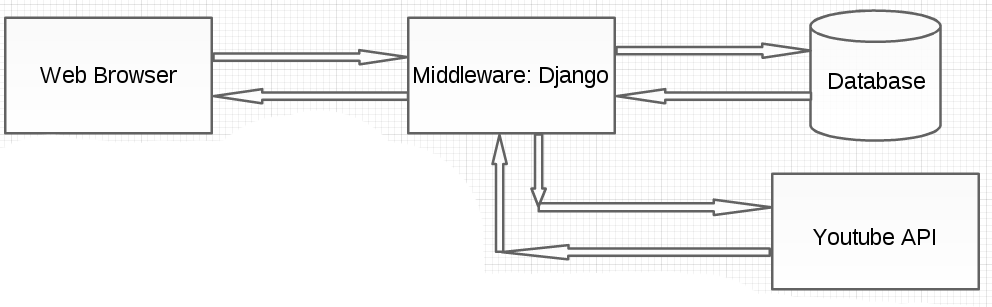
\includegraphics[width=0.45\textwidth]{ntier}
    \caption{N-Tier Diagram} \label{fig:n-tier}
  \end{center}
\end{figure}

\begin{figure}[h]
  \begin{center}
    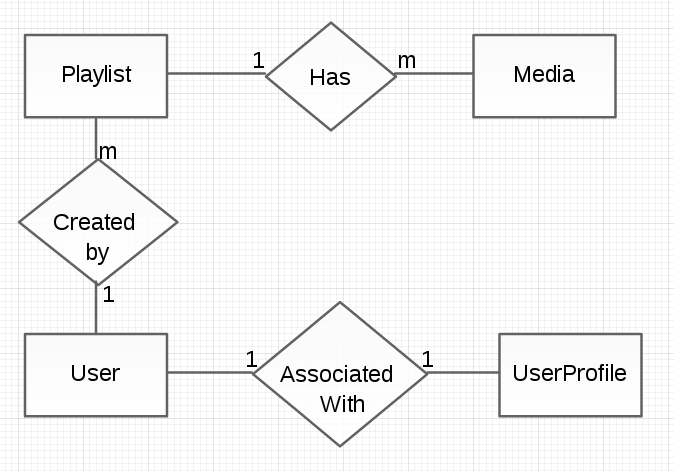
\includegraphics[width=0.45\textwidth]{ER}
    \caption{Entity-Relationship Diagram} \label{fig:ER}
  \end{center}
\end{figure}

